\documentclass{standalone}
\usepackage{tikz}
\usetikzlibrary{patterns, positioning}
\usetikzlibrary{shapes.misc}
\usepackage[outline]{contour}
\contourlength{1.5pt} 
\usepackage[sfdefault]{ClearSans} %% option 'sfdefault' activates Clear Sans as the default text font
\usepackage[T1]{fontenc}

\begin{document}
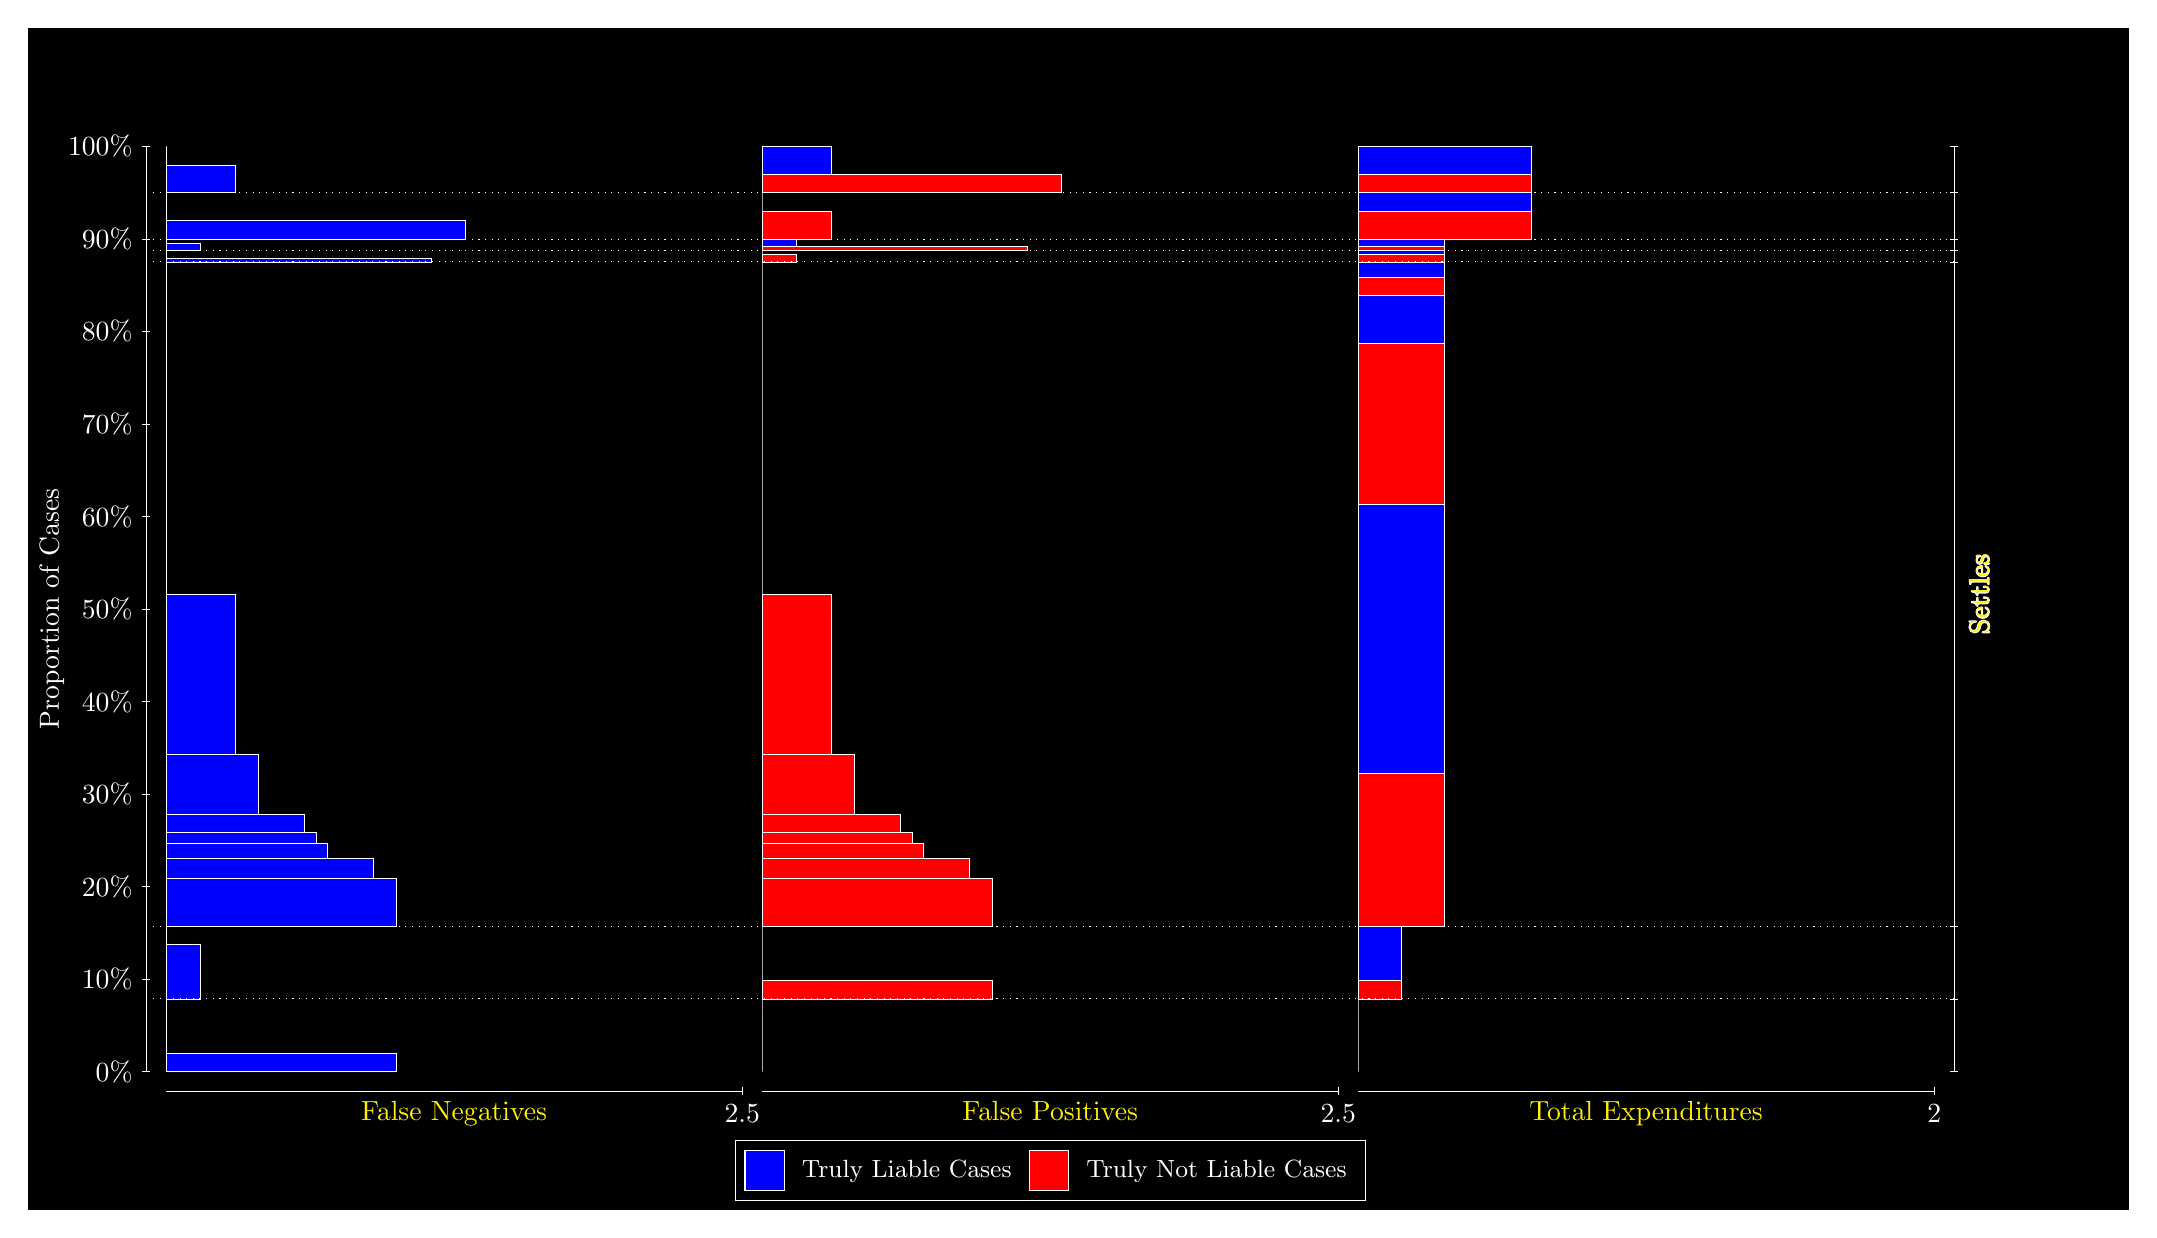
\begin{tikzpicture}
\draw[fill=black] (0,0) rectangle (26.667,15);
\draw[white, very thin] (1.5,1.75) -- (1.5,13.5);
\node[rotate=90, text=white, anchor=center] at (0.3, 7.625) {Proportion of Cases};
\draw[white, very thin] (1.45,1.75) -- (1.55,1.75);
\node[text=white, anchor=east] at (1.45, 1.75) {0\%};
\draw[white, very thin] (1.45,2.925) -- (1.55,2.925);
\node[text=white, anchor=east] at (1.45, 2.925) {10\%};
\draw[white, very thin] (1.45,4.1) -- (1.55,4.1);
\node[text=white, anchor=east] at (1.45, 4.1) {20\%};
\draw[white, very thin] (1.45,5.275) -- (1.55,5.275);
\node[text=white, anchor=east] at (1.45, 5.275) {30\%};
\draw[white, very thin] (1.45,6.45) -- (1.55,6.45);
\node[text=white, anchor=east] at (1.45, 6.45) {40\%};
\draw[white, very thin] (1.45,7.625) -- (1.55,7.625);
\node[text=white, anchor=east] at (1.45, 7.625) {50\%};
\draw[white, very thin] (1.45,8.8) -- (1.55,8.8);
\node[text=white, anchor=east] at (1.45, 8.8) {60\%};
\draw[white, very thin] (1.45,9.975) -- (1.55,9.975);
\node[text=white, anchor=east] at (1.45, 9.975) {70\%};
\draw[white, very thin] (1.45,11.15) -- (1.55,11.15);
\node[text=white, anchor=east] at (1.45, 11.15) {80\%};
\draw[white, very thin] (1.45,12.325) -- (1.55,12.325);
\node[text=white, anchor=east] at (1.45, 12.325) {90\%};
\draw[white, very thin] (1.45,13.5) -- (1.55,13.5);
\node[text=white, anchor=east] at (1.45, 13.5) {100\%};

\draw[white, very thin] (24.457,1.75) -- (24.457,13.5);
\draw[white, very thin] (24.407,1.75) -- (24.507,1.75);
\node[anchor=west] at (24.407, 1.75) {};
\draw[white, very thin] (24.407,2.6722) -- (24.507,2.6722);
\node[anchor=west] at (24.407, 2.6722) {};
\draw[white, very thin] (24.407,3.5943) -- (24.507,3.5943);
\node[anchor=west] at (24.407, 3.5943) {};
\draw[white, very thin] (24.407,12.032) -- (24.507,12.032);
\node[anchor=west] at (24.407, 12.032) {};
\draw[white, very thin] (24.407,12.177) -- (24.507,12.177);
\node[anchor=west] at (24.407, 12.177) {};
\draw[white, very thin] (24.407,12.321) -- (24.507,12.321);
\node[anchor=west] at (24.407, 12.321) {};
\draw[white, very thin] (24.407,12.911) -- (24.507,12.911);
\node[anchor=west] at (24.407, 12.911) {};
\draw[white, very thin] (24.407,13.5) -- (24.507,13.5);
\node[anchor=west] at (24.407, 13.5) {};

\draw[white, very thin, fill=blue] (1.75,1.75) rectangle (4.6775,1.9822);
\draw[white, very thin, fill=red] (1.75,1.9822) rectangle (1.75,2.6722);
\draw[white, very thin, fill=blue] (1.75,2.6722) rectangle (2.1891,3.3621);
\draw[white, very thin, fill=red] (1.75,3.3621) rectangle (1.75,3.5943);
\draw[white, very thin, fill=blue] (1.75,3.5943) rectangle (4.6775,4.2072);
\draw[white, very thin, fill=blue] (1.75,4.2072) rectangle (4.3848,4.4584);
\draw[white, very thin, fill=blue] (1.75,4.4584) rectangle (3.7993,4.6481);
\draw[white, very thin, fill=blue] (1.75,4.6481) rectangle (3.6529,4.7877);
\draw[white, very thin, fill=blue] (1.75,4.7877) rectangle (3.5065,5.0215);
\draw[white, very thin, fill=blue] (1.75,5.0215) rectangle (2.921,5.7746);
\draw[white, very thin, fill=blue] (1.75,5.7746) rectangle (2.6283,7.8132);
\draw[white, very thin, fill=red] (1.75,7.8132) rectangle (1.75,12.032);
\draw[white, very thin, fill=blue] (1.75,12.032) rectangle (5.1167,12.083);
\draw[white, very thin, fill=red] (1.75,12.083) rectangle (1.75,12.177);
\draw[white, very thin, fill=blue] (1.75,12.177) rectangle (2.1891,12.271);
\draw[white, very thin, fill=red] (1.75,12.271) rectangle (1.75,12.321);
\draw[white, very thin, fill=blue] (1.75,12.321) rectangle (5.5558,12.556);
\draw[white, very thin, fill=red] (1.75,12.556) rectangle (1.75,12.911);
\draw[white, very thin, fill=blue] (1.75,12.911) rectangle (2.6283,13.265);
\draw[white, very thin, fill=red] (1.75,13.265) rectangle (1.75,13.5);
\draw[white, very thin, fill=red] (9.3189,1.75) rectangle (9.3189,2.44);
\draw[white, very thin, fill=blue] (9.3189,2.44) rectangle (9.3189,2.6722);
\draw[white, very thin, fill=red] (9.3189,2.6722) rectangle (12.246,2.9044);
\draw[white, very thin, fill=blue] (9.3189,2.9044) rectangle (9.3189,3.5943);
\draw[white, very thin, fill=red] (9.3189,3.5943) rectangle (12.246,4.2072);
\draw[white, very thin, fill=red] (9.3189,4.2072) rectangle (11.954,4.4584);
\draw[white, very thin, fill=red] (9.3189,4.4584) rectangle (11.368,4.6481);
\draw[white, very thin, fill=red] (9.3189,4.6481) rectangle (11.222,4.7876);
\draw[white, very thin, fill=red] (9.3189,4.7876) rectangle (11.075,5.0215);
\draw[white, very thin, fill=red] (9.3189,5.0215) rectangle (10.49,5.7746);
\draw[white, very thin, fill=red] (9.3189,5.7746) rectangle (10.197,7.8134);
\draw[white, very thin, fill=blue] (9.3189,7.8134) rectangle (9.3189,12.032);
\draw[white, very thin, fill=red] (9.3189,12.032) rectangle (9.758,12.127);
\draw[white, very thin, fill=blue] (9.3189,12.127) rectangle (9.3189,12.177);
\draw[white, very thin, fill=red] (9.3189,12.177) rectangle (12.686,12.227);
\draw[white, very thin, fill=blue] (9.3189,12.227) rectangle (9.758,12.321);
\draw[white, very thin, fill=red] (9.3189,12.321) rectangle (10.197,12.676);
\draw[white, very thin, fill=blue] (9.3189,12.676) rectangle (9.3189,12.911);
\draw[white, very thin, fill=red] (9.3189,12.911) rectangle (13.125,13.146);
\draw[white, very thin, fill=blue] (9.3189,13.146) rectangle (10.197,13.5);
\draw[white, very thin, fill=red] (16.888,1.75) rectangle (16.888,2.44);
\draw[white, very thin, fill=blue] (16.888,2.44) rectangle (16.888,2.6722);
\draw[white, very thin, fill=red] (16.888,2.6722) rectangle (17.437,2.9044);
\draw[white, very thin, fill=blue] (16.888,2.9044) rectangle (17.437,3.5943);
\draw[white, very thin, fill=red] (16.888,3.5943) rectangle (17.986,5.5407);
\draw[white, very thin, fill=blue] (16.888,5.5407) rectangle (17.986,8.957);
\draw[white, very thin, fill=red] (16.888,8.957) rectangle (17.986,10.996);
\draw[white, very thin, fill=blue] (16.888,10.996) rectangle (17.986,11.609);
\draw[white, very thin, fill=red] (16.888,11.609) rectangle (17.986,11.843);
\draw[white, very thin, fill=blue] (16.888,11.843) rectangle (17.986,12.032);
\draw[white, very thin, fill=red] (16.888,12.032) rectangle (17.986,12.127);
\draw[white, very thin, fill=blue] (16.888,12.127) rectangle (17.986,12.177);
\draw[white, very thin, fill=red] (16.888,12.177) rectangle (17.986,12.227);
\draw[white, very thin, fill=blue] (16.888,12.227) rectangle (17.986,12.321);
\draw[white, very thin, fill=red] (16.888,12.321) rectangle (19.083,12.676);
\draw[white, very thin, fill=blue] (16.888,12.676) rectangle (19.083,12.911);
\draw[white, very thin, fill=red] (16.888,12.911) rectangle (19.083,13.146);
\draw[white, very thin, fill=blue] (16.888,13.146) rectangle (19.083,13.5);
\draw[white, dotted] (1.5,2.6722) -- (24.457,2.6722);
\draw[white, dotted] (1.5,3.5943) -- (24.457,3.5943);
\draw[white, dotted] (1.5,12.032) -- (24.457,12.032);
\draw[white, dotted] (1.5,12.177) -- (24.457,12.177);
\draw[white, dotted] (1.5,12.321) -- (24.457,12.321);
\draw[white, dotted] (1.5,12.911) -- (24.457,12.911);
\draw[white, very thin] (1.75,1.5) -- (9.0689,1.5);
\node[text=yellow, anchor=north] at (5.4094, 1.5) {False Negatives};
\draw[white, very thin] (9.0689,1.45) -- (9.0689,1.55);
\node[text=white, anchor=north] at (9.0689, 1.45) {2.5};

\draw[white, very thin] (9.3189,1.5) -- (16.638,1.5);
\node[text=yellow, anchor=north] at (12.978, 1.5) {False Positives};
\draw[white, very thin] (16.638,1.45) -- (16.638,1.55);
\node[text=white, anchor=north] at (16.638, 1.45) {2.5};

\draw[white, very thin] (16.888,1.5) -- (24.207,1.5);
\node[text=yellow, anchor=north] at (20.547, 1.5) {Total Expenditures};
\draw[white, very thin] (24.207,1.45) -- (24.207,1.55);
\node[text=white, anchor=north] at (24.207, 1.45) {2};



\node[text=yellow, centered, rotate=90] at (24.777, 7.8133) {\contour{white}{Settles}};





\draw (12.978300999999998,1.5) node[draw=none] (baseCoordinate) {};
\begin{scope}[align=center]
        \matrix[scale=0.5, draw=white, below=0.5cm of baseCoordinate, nodes={draw}, column sep=0.1cm]{
            \node[rectangle, draw, minimum width=0.5cm, minimum height=0.5cm, fill=blue] {}; &
            \node[draw=none, font=\small, text=white] (B) {Truly Liable Cases}; &
            \node[rectangle, draw, minimum width=0.5cm, minimum height=0.5cm, fill=red] {}; &
            \node[draw=none, font=\small, text=white] (B) {Truly Not Liable Cases}; \\
            };
\end{scope}

\end{tikzpicture}
\end{document}